\section{Sơ đồ Ca sử dụng Tổng thể Toàn hệ thống}
\label{sec:system_usecase}

\begin{figure}[H]
    \centering
    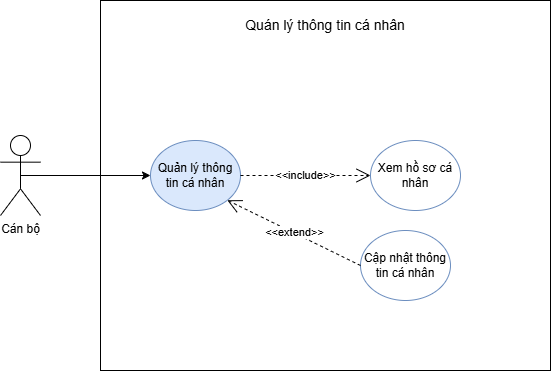
\includegraphics[width=0.9\linewidth]{img/uml/system_usecase_diagram.png}
    \caption{\textit{Sơ đồ Ca sử dụng Tổng thể Hệ thống MyHCMUT}}
    \label{fig:usecase_overall}
\end{figure}

\section{Bảng Đặc tả Chi tiết các Ca sử dụng Cốt lõi}
\label{sec:dacta_usecase_chitiet}

\subsection{UC01: Tra cứu \& Đề xuất Thẩm định Chỉnh sửa Lý lịch Cán bộ}
\begin{table}[H]
\centering
\renewcommand{\arraystretch}{1.2}
\begin{tabularx}{\textwidth}{|p{3.2cm}|X|}
\hline
\textbf{Tên Ca sử dụng} & \textbf{UC01: Tra cứu \& Đề xuất Thẩm định Chỉnh sửa Lý lịch Cán bộ} \\
\hline
\textbf{Tác nhân} & Cán bộ/Giảng viên (Người gửi), Chuyên viên Phòng TCCB (Người duyệt) \\
\hline
\textbf{Tiền điều kiện} & Cán bộ đã đăng nhập thành công vào ứng dụng MyHCMUT. \\
\hline
\textbf{Hậu điều kiện} & Dữ liệu hồ sơ lý lịch được cập nhật chính thức vào cơ sở dữ liệu nhân sự. \\
\hline
\textbf{Luồng sự kiện chính} & 
1. Cán bộ mở màn hình \texttt{PersonalProfilePage}, xem 11 tab lý lịch chi tiết. \newline
2. Cán bộ chọn mục cần chỉnh sửa, nhập giá trị mới và đính kèm ảnh minh chứng. \newline
3. Nhấn nút \textit{``Gửi đề xuất''} $\rightarrow$ Hệ thống lưu vào bảng \texttt{staff\_ly\_lich\_request} (trạng thái \texttt{PENDING}) và đẩy thông báo cho Phòng TCCB. \newline
4. Chuyên viên TCCB mở màn hình \texttt{ApproveProfileDetailPage}, xem giao diện Diff Viewer so sánh trực quan giá trị cũ (màu đỏ) và giá trị mới (màu xanh). \newline
5. Chuyên viên chọn \textit{``Duyệt''} $\rightarrow$ Hệ thống ghi đè dữ liệu mới vào \texttt{staff\_ly\_lich} và gửi thông báo hoàn tất cho Cán bộ. \\
\hline
\textbf{Luồng ngoại lệ} & Nếu Chuyên viên chọn \textit{``Từ chối''}, bắt buộc nhập lý do $\rightarrow$ Đề xuất chuyển trạng thái \texttt{REJECTED} và thông báo cho Cán bộ. \\
\hline
\end{tabularx}
\caption{\textit{Đặc tả Ca sử dụng UC01: Tra cứu và Thẩm định Sửa Lý lịch}}
\label{tab:uc01_profile}
\end{table}

\subsection{UC02: Đăng ký Nghỉ phép (Form Wizard 4 bước \& Real-time Validation)}
\begin{table}[H]
\centering
\renewcommand{\arraystretch}{1.2}
\begin{tabularx}{\textwidth}{|p{3.2cm}|X|}
\hline
\textbf{Tên Ca sử dụng} & \textbf{UC02: Đăng ký Nghỉ phép với Kiểm tra Ràng buộc Thời gian thực} \\
\hline
\textbf{Tác nhân} & Cán bộ / Giảng viên \\
\hline
\textbf{Tiền điều kiện} & Cán bộ đã đăng nhập; còn tài khoản hoạt động trong hệ thống. \\
\hline
\textbf{Hậu điều kiện} & Đơn nghỉ phép được tạo thành công ở trạng thái \texttt{CHO\_DUYET} và kích hoạt quy trình phê duyệt. \\
\hline
\textbf{Luồng sự kiện chính} & 
1. Cán bộ mở màn hình \texttt{LeaveRequestPage}, bắt đầu Bước 1: Chọn loại nghỉ và lý do. \newline
2. Bước 2: Chọn khoảng thời gian (Từ ngày $\rightarrow$ Đến ngày). \newline
3. Hệ thống tự động gọi API \texttt{/api/tcns-nghi-phep/validate} để thực thi 4 tầng kiểm tra: (a) Tính số ngày làm việc thực tế, (b) Kiểm tra trùng lịch cá nhân, (c) Kiểm tra mốc nộp trễ 3 ngày/15 ngày, (d) Kiểm tra số dư quỹ phép năm. \newline
4. Nếu nộp trễ hạn quy định $\rightarrow$ Bước 3 yêu cầu bắt buộc nhập lý do giải trình trễ. \newline
5. Bước 4: Cán bộ xác nhận cam kết bàn giao công việc và nhấn nút \textit{``Gửi duyệt''}. \newline
6. Hệ thống lưu bản ghi vào \texttt{tcns\_nghi\_phep\_dang\_ky} và đẩy thông báo tới Lãnh đạo Đơn vị. \\
\hline
\textbf{Luồng ngoại lệ} & Nếu số ngày nghỉ vượt quá quỹ phép năm hoặc trùng lịch công tác $\rightarrow$ Hệ thống báo lỗi và không cho phép chuyển tiếp sang bước tiếp theo. \\
\hline
\end{tabularx}
\caption{\textit{Đặc tả Ca sử dụng UC02: Đăng ký Nghỉ phép}}
\label{tab:uc02_leave}
\end{table}

\subsection{UC03: Đăng ký \& Phê duyệt Đi công tác (Business Trip Workflow)}
\begin{table}[H]
\centering
\renewcommand{\arraystretch}{1.2}
\begin{tabularx}{\textwidth}{|p{3.2cm}|X|}
\hline
\textbf{Tên Ca sử dụng} & \textbf{UC03: Đăng ký và Phê duyệt Chuyến Đi công tác} \\
\hline
\textbf{Tác nhân} & Cán bộ đăng ký, Lãnh đạo Đơn vị, Ban Giám hiệu / Phòng TCCB \\
\hline
\textbf{Tiền điều kiện} & Cán bộ có kế hoạch đi công tác trong hoặc ngoài nước. \\
\hline
\textbf{Hậu điều kiện} & Quyết định cử cán bộ đi công tác được phê duyệt và lưu vào lịch trình công tác. \\
\hline
\textbf{Luồng sự kiện chính} & 
1. Cán bộ mở màn hình \texttt{BusinessTripEditPage}, điền mục đích, địa điểm, thời gian, phương tiện di chuyển, dự toán kinh phí và chọn thành viên đoàn công tác. \newline
2. Đính kèm tệp PDF thư mời/kế hoạch công tác $\rightarrow$ Nhấn \textit{``Gửi duyệt''}. \newline
3. Lãnh đạo Đơn vị nhận thông báo đẩy FCM, mở \texttt{ApproveBtripListPage} xem xét chi tiết chuyến đi $\rightarrow$ Chọn \textit{``Phê duyệt''}. \newline
4. Nếu chuyến công tác yêu cầu phê duyệt cấp trường $\rightarrow$ Hệ thống chuyển tiếp lên BGH/Phòng TCCB duyệt và cấp số quyết định. \newline
5. Hệ thống cập nhật trạng thái \texttt{DA\_DUYET} và thông báo tới toàn bộ thành viên đoàn công tác. \\
\hline
\end{tabularx}
\caption{\textit{Đặc tả Ca sử dụng UC03: Đăng ký và Phê duyệt Đi công tác}}
\label{tab:uc03_btrip}
\end{table}

\subsection{UC04: Quản lý \& Giám sát Tiến độ Nhiệm vụ/Công việc (Tasks/Missions)}
\begin{table}[H]
\centering
\renewcommand{\arraystretch}{1.2}
\begin{tabularx}{\textwidth}{|p{3.2cm}|X|}
\hline
\textbf{Tên Ca sử dụng} & \textbf{UC04: Quản lý và Giám sát Tiến độ Nhiệm vụ} \\
\hline
\textbf{Tác nhân} & Cán bộ phụ trách, Lãnh đạo Đơn vị, Ban Giám hiệu \\
\hline
\textbf{Tiền điều kiện} & Nhiệm vụ đã được khởi tạo trên hệ thống điều hành của Nhà trường. \\
\hline
\textbf{Hậu điều kiện} & Cán bộ cập nhật tiến độ công việc và gửi báo cáo đợt thành công. \\
\hline
\textbf{Luồng sự kiện chính} & 
1. Người dùng mở \texttt{MissionsListPage}, lọc theo loại nhiệm vụ (Trọng tâm, Được giao, Chung) và trạng thái (Cần xử lý, Đang làm, Đã xong). \newline
2. Chọn một nhiệm vụ cụ thể $\rightarrow$ Mở màn hình \texttt{MissionDetailPage} với 4 tab: (a) Tổng quan \% tiến độ \& hạn chót, (b) Cây đầu việc phân cấp (\texttt{outlined-tree}), (c) Báo cáo tiến độ các đợt, (d) Văn bản liên kết. \newline
3. Cán bộ nhấn vào một công việc cụ thể $\rightarrow$ Mở \texttt{TaskDetailBottomSheet} để xem người thực hiện và checklist. \newline
4. Cán bộ gửi đợt báo cáo tiến độ kèm tệp minh chứng $\rightarrow$ Hệ thống ghi nhận và cập nhật tỷ lệ hoàn thành chung của nhiệm vụ. \\
\hline
\end{tabularx}
\caption{\textit{Đặc tả Ca sử dụng UC04: Quản lý và Giám sát Nhiệm vụ}}
\label{tab:uc04_mission}
\end{table}

\subsection{UC05: Điểm danh Cuộc họp Thời gian thực \& Báo vắng (Real-time Attendance)}
\begin{table}[H]
\centering
\renewcommand{\arraystretch}{1.2}
\begin{tabularx}{\textwidth}{|p{3.2cm}|X|}
\hline
\textbf{Tên Ca sử dụng} & \textbf{UC05: Điểm danh Cuộc họp Thời gian thực và Báo vắng} \\
\hline
\textbf{Tác nhân} & Cán bộ tham dự cuộc họp, Ban Tổ chức cuộc họp \\
\hline
\textbf{Tiền điều kiện} & Cuộc họp đã được ban hành trong Lịch tuần trường hoặc Lịch đơn vị. \\
\hline
\textbf{Hậu điều kiện} & Trạng thái có mặt/báo vắng của đại biểu được cập nhật thời gian thực tới toàn bộ hệ thống. \\
\hline
\textbf{Luồng sự kiện chính} & 
1. Cán bộ mở màn hình \texttt{ScheduleView}, chọn cuộc họp trong ngày. \newline
2. Ứng dụng kiểm tra ràng buộc khung giờ: từ trước giờ họp 1 giờ đến hết ngày diễn ra cuộc họp. \newline
3. Nút \textit{``Điểm danh có mặt''} sáng lên $\rightarrow$ Cán bộ nhấn nút. \newline
4. Hệ thống gọi API \texttt{/api/schedule/general-item/:id/checkin}, ghi nhận vào cơ sở dữ liệu và phát sự kiện WebSocket (\texttt{Socket.IO: scheduleCheckin}). \newline
5. Màn hình của Ban tổ chức và các đại biểu khác tự động cập nhật danh sách có mặt tức thời. \newline
6. Nếu vắng mặt, cán bộ nhấn \textit{``Báo vắng''} và nhập lý do (1--200 ký tự) $\rightarrow$ Hệ thống đồng bộ trạng thái vắng có lý do. \\
\hline
\end{tabularx}
\caption{\textit{Đặc tả Ca sử dụng UC05: Điểm danh Cuộc họp Thời gian thực}}
\label{tab:uc05_attendance}
\end{table}